\documentclass[25pt, a0paper, portrait, margin=0mm, innermargin=15mm,
               blockverticalspace=12mm, colspace=15mm, subcolspace=8mm]{tikzposter}

\usepackage{amsmath, amssymb, bm}
\usepackage{graphicx}
\usepackage{booktabs}
\usepackage{enumitem}
\setlist{leftmargin=*, nosep, itemsep=3pt}

\graphicspath{{../figures/}}

% ---- Custom Dartmouth-green theme ----
\definecolor{dartgreen}{HTML}{0B4F2F}
\definecolor{dartlight}{HTML}{E8F0EC}
\definecolor{accent}{HTML}{7A1F8B}

\definecolorstyle{DartmouthStyle}{
  \definecolor{colorOne}{HTML}{0B4F2F}
  \definecolor{colorTwo}{HTML}{E8F0EC}
  \definecolor{colorThree}{HTML}{7A1F8B}
}{
  \colorlet{backgroundcolor}{white}
  \colorlet{framecolor}{dartgreen}
  \colorlet{titlefgcolor}{white}
  \colorlet{titlebgcolor}{dartgreen}
  \colorlet{blocktitlebgcolor}{dartgreen}
  \colorlet{blocktitlefgcolor}{white}
  \colorlet{blockbodybgcolor}{white}
  \colorlet{blockbodyfgcolor}{black}
  \colorlet{innerblocktitlebgcolor}{dartlight}
  \colorlet{innerblocktitlefgcolor}{dartgreen}
  \colorlet{notebgcolor}{dartlight}
  \colorlet{notefgcolor}{black}
}

\usetheme{Default}
\usecolorstyle{DartmouthStyle}
\usetitlestyle{Filled}
\useblockstyle{Default}

\title{\parbox{\linewidth}{\centering Sparse, Low-Rank, and Deep:\\[6pt]
A Compressed-Sensing Framework for Music Source Separation}}
\author{Taka Khoo}
\institute{Thayer School of Engineering, Dartmouth College \quad$\cdot$\quad
ENGS 109: High-Dimensional Sensing and Learning (Spring 2026)}

\begin{document}
\maketitle

\begin{columns}

% ================= LEFT COLUMN =================
\column{0.34}

\block{The problem, and why it is personal}{
\textbf{Music source separation} splits a finished mix into stems (vocals,
accompaniment). It is the suggested project bullet \emph{``isolate instrumental
music from vocal component,''} and it is the third time I have studied audio
under Peter Chin:
\begin{itemize}
\item[\textcolor{dartgreen}{\textbf{I}}] \textbf{Undergrad thesis:} a 1.08B-param
Token U-Net for full-mix \emph{restoration} on EnCodec tokens.
\item[\textcolor{dartgreen}{\textbf{II}}] \textbf{MS thesis:} MODULO / Mozart AI,
a co-creative DAW whose stem \emph{separation} is outsourced to ElevenLabs
($\approx$35 dB SI-SDR below Demucs).
\item[\textcolor{accent}{\textbf{III}}] \textbf{This project:} attack separation
from the compressed-sensing angle, with the recovery theory the deep baselines lack.
\end{itemize}
}

\block{Music separation \textit{is} compressed sensing}{
On the STFT magnitude $\bm{M}=|\mathrm{STFT}(y)|$:
\begin{itemize}
\item Vocals are \textbf{sparse in frequency} (thin formants); drums
\textbf{sparse in time} (transients).
\item Sustained harmony is \textbf{low-rank} (L13).
\item Stereo channels share active sources: \textbf{joint sparsity / MMV} (L12).
\item Deep nets work because they \textbf{unroll sparse coding} (L16).
\end{itemize}
\vspace{4pt}
\begin{tikzfigure}
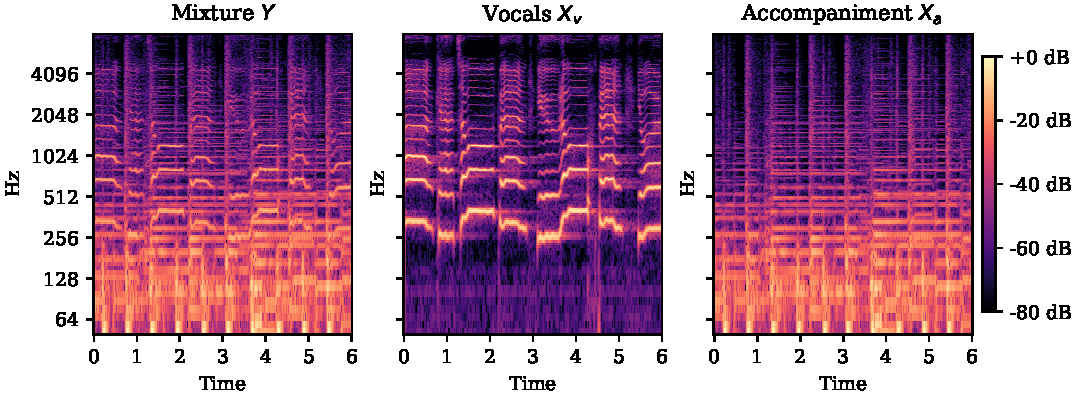
\includegraphics[width=0.96\linewidth]{fig_triptych.pdf}
\end{tikzfigure}
\textit{\small Mixture vs. vocals vs. accompaniment. The structure each stage exploits.}
}

\block{Stage A: Robust PCA (L13)}{
\[ \min_{\bm{X},\bm{E}} \ \|\bm{X}\|_* + \lambda\|\bm{E}\|_1 \ \text{ s.t. } \
\bm{M}=\bm{X}+\bm{E}, \quad \lambda=\tfrac{1}{\sqrt{\max(F,T)}} \]
Low-rank $\bm{X}$ = accompaniment, sparse $\bm{E}$ = transients. Training-free,
inexact ALM, converges to $10^{-7}$ in 38 iterations.
\begin{tikzfigure}
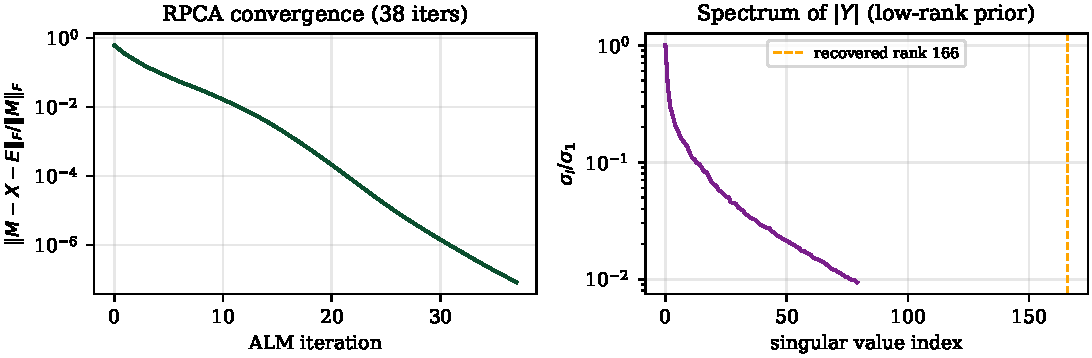
\includegraphics[width=0.96\linewidth]{fig_rpca_converge.pdf}
\end{tikzfigure}
}

% ================= MIDDLE COLUMN =================
\column{0.34}

\block{Stage D: SparseNet for spectrograms (L16)}{
\textbf{The novel contribution.} Chin's SparseNet has only been tested on image
classification. We adapt its \textbf{composite sparse-coding module} to
\textbf{audio mask regression}. Each module maps a magnitude frame
$\bm{x}\in\mathbb{R}^F$ through two non-negative sparse codes:
\[ \bm{\alpha}^{(1)}=\arg\min_{\bm{\alpha}\ge0}\tfrac12\|\bm{x}-\bm{D}^{(1)}\bm{\alpha}\|_2^2
+\lambda_1\|\bm{\alpha}\|_1+\tfrac{\lambda_2}2\|\bm{\alpha}\|_2^2 \]
\[ \bm{\alpha}^{(2)}=\arg\min_{\bm{\alpha}\ge0}\tfrac12\|\bm{\alpha}^{(1)}
-\bm{D}^{(2)}\bm{\alpha}\|_2^2+\lambda_1\|\bm{\alpha}\|_1+\tfrac{\lambda_2}2\|\bm{\alpha}\|_2^2 \]
with $\bm{D}^{(1)}$ \emph{fat} (upsampling) and $\bm{D}^{(2)}$ \emph{tall}
(downsampling). We \textbf{unroll 25 steps of non-negative FISTA} per code and
train 3 stacked modules \textbf{end-to-end by backprop} on Apple MPS. Dictionaries
and shrinkage parameters are learned; the head emits a soft mask.
\begin{tikzfigure}
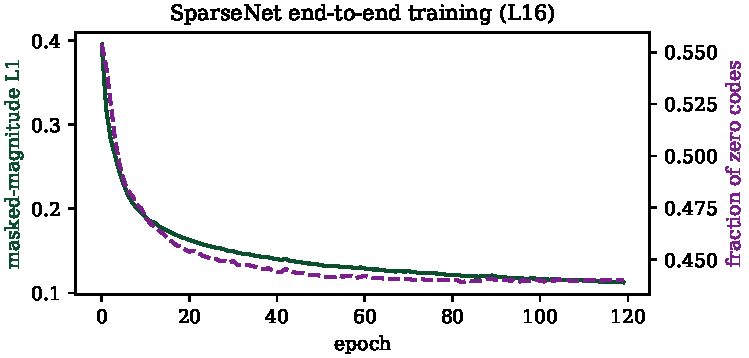
\includegraphics[width=0.95\linewidth]{fig_sparsenet_train.pdf}
\end{tikzfigure}
\textit{\small Codes stay $\sim$44\% sparse throughout end-to-end training.}
}

\block{The five-stage pipeline}{
\begin{center}
\begin{tabular}{@{}cll@{}}
\toprule
\textbf{Stage} & \textbf{Method} & \textbf{Lecture} \\
\midrule
A & Robust PCA (low-rank + sparse) & L13 \\
B & Class-conditional NMF & L15 \\
C & K-SVD dictionaries + SRC & L14, L8 \\
D & \textbf{SparseNet mask predictor} & \textbf{L16} \\
E & MMV joint sparsity (stereo) & L12 \\
\bottomrule
\end{tabular}
\end{center}
\vspace{3pt}
Every stage reuses problem-set code: OMP (PS3), FISTA (PS5), SRC (PS7),
nuclear-norm SVT (PS8).
}

\block{Learned dictionaries (L14, L15)}{
\begin{tikzfigure}
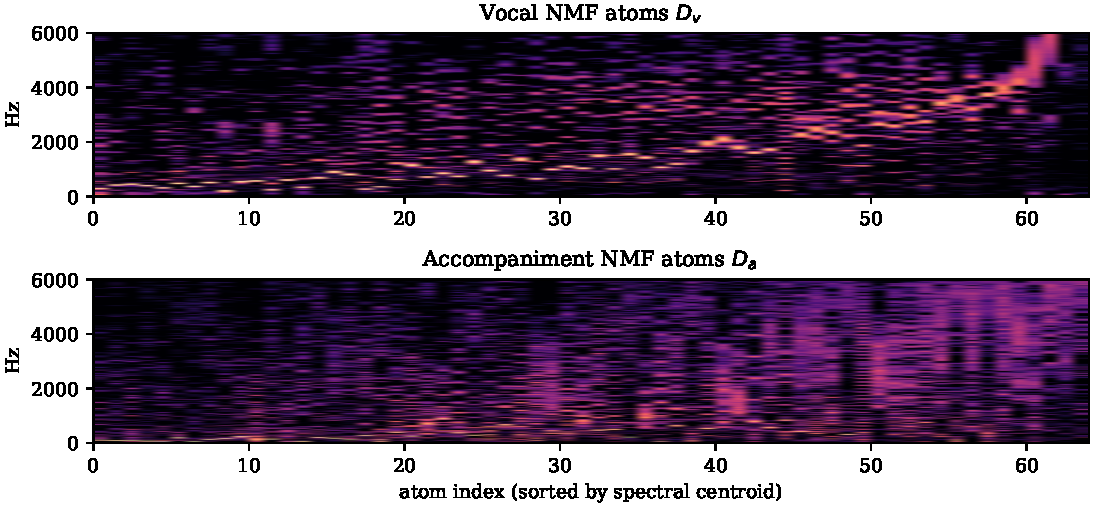
\includegraphics[width=0.96\linewidth]{fig_nmf_atoms.pdf}
\end{tikzfigure}
\textit{\small Vocal atoms ride the formant region; accompaniment atoms spread
lower. Parts-based, exactly the L15 prediction.}
}

% ================= RIGHT COLUMN =================
\column{0.32}

\block{Results: MUSDB18 sample}{
\begin{center}
\begin{tabular}{@{}llcc@{}}
\toprule
\textbf{Stage} & \textbf{Lec.} & \textbf{Voc.} & \textbf{Acc.} \\
\midrule
A. Robust PCA   & L13 & $-3.6$ & $0.1$ \\
B. NMF (KL)     & L15 & $1.3$  & $6.9$ \\
C. K-SVD + SRC  & L14/8 & $\mathbf{2.7}$ & $7.2$ \\
D. SparseNet    & L16 & $2.5$ & $\mathbf{8.2}$ \\
\midrule
Oracle (IRM)    & --- & $10.1$ & $15.5$ \\
\bottomrule
\end{tabular}
\end{center}
\small Median SI-SDR (dB), 12 held-out tracks.
\begin{tikzfigure}
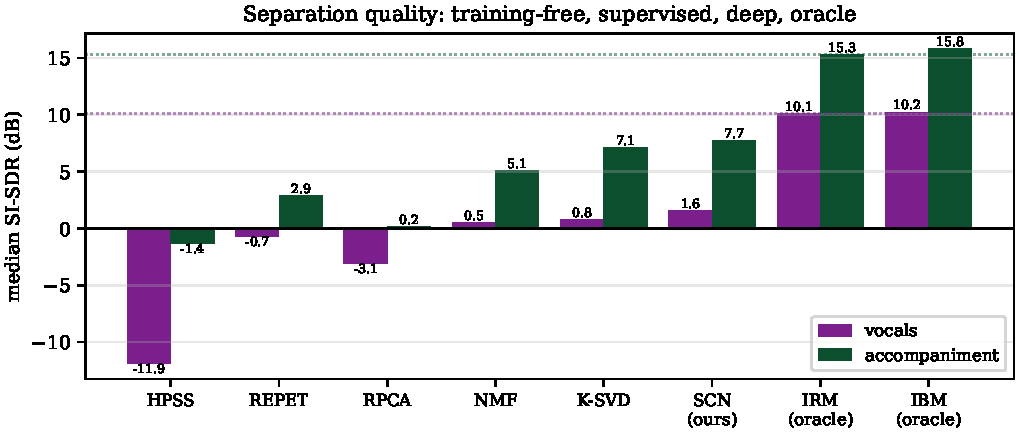
\includegraphics[width=0.98\linewidth]{fig_results_bars.pdf}
\end{tikzfigure}
\textbf{Clean unsupervised$\to$supervised$\to$deep progression.} SparseNet matches
discriminative K-SVD on vocals and leads on accompaniment.
}

\block{An honest negative result}{
\begin{tikzfigure}
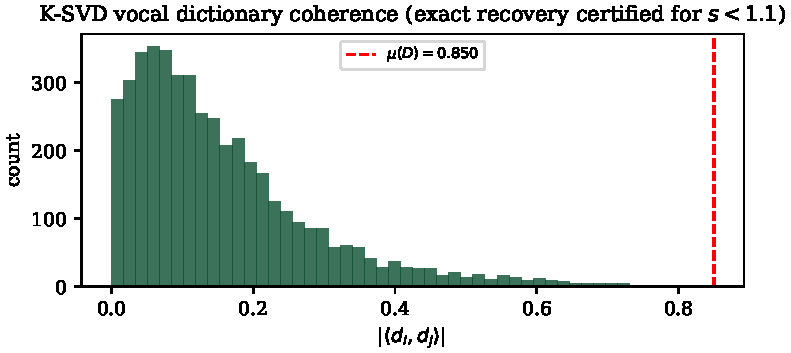
\includegraphics[width=0.96\linewidth]{fig_ksvd_coherence.pdf}
\end{tikzfigure}
Learned K-SVD dictionaries have coherence $\mu\!\approx\!0.85$. The L7 worst-case
guarantee then certifies only $S\!\lesssim\!1$, yet OMP at $S\!=\!10$ works well.
\textbf{Average-case $\ne$ worst-case} for trained dictionaries.
}

\block{Takeaways}{
\begin{itemize}
\item Five course methods, one evaluable spectrogram pipeline.
\item First adaptation of \textbf{SparseNet to audio mask regression} (L16).
\item Theory (RIP, coherence, RPCA $\lambda\!=\!1/\sqrt{N_1}$) connected to every stage,
\textbf{including where it goes slack}.
\item All code, trained weights, and \textbf{playable audio} released.
\end{itemize}
\vspace{4pt}
\centering
\textbf{\textcolor{dartgreen}{github.com/takakhoo/ENGS109\_Final\_Project}}
}

\end{columns}

\end{document}
